\documentclass[12pt,a4paper]{article}
%\usepackage{geometry}[paper=a4paper,left=30mm,width=150mm,top=25mm,bottom=25mm]
\usepackage[margin=2cm]{geometry}
\usepackage[utf8]{inputenc}
\usepackage{amsmath}
\usepackage{amsfonts}
\usepackage{amssymb}
\usepackage[pdftex]{graphicx}
\begin{document}
\author{Timothy Trewartha \\
\and
Michiel Johan Baird \\
\and
Supervisor: Hussein Suleman \\
Department of Computer Science \\
University of Cape Town
 }
\title{Display and Management of Geomatics Research Data}
\maketitle

\section{Project Description}
The Zamani project, started by the UCT Department of Geomatics, aims to
preserve African cultural heritage by documenting heritage sites and producing
laser scanned models. Currently they have documented about 40 sites in 12 African
countries with close to 100 models. Some of the models are very detailed, containing
billions of points. With a fast-growing volume of data, the Department of Geomatics
is facing several challenges, ranging from basic storage of the data to viewing and
interacting with the large models in real-time.

There are two main components to this project. The first is to develop a system to
enable both viewing and streaming of the Zamani models in their full detail, at
interactive frame rates. The second is to investigate various ways of automating
GIS (Geographic Information Systems) workflow. The aim is to develop a software tool
to enable more efficient manipulation of GIS data. The real-time streaming
infrastructure will additionally be integrated into the software developed for
workflow automation, as shown in the following diagram.
\begin{figure}[h!]
\centering
    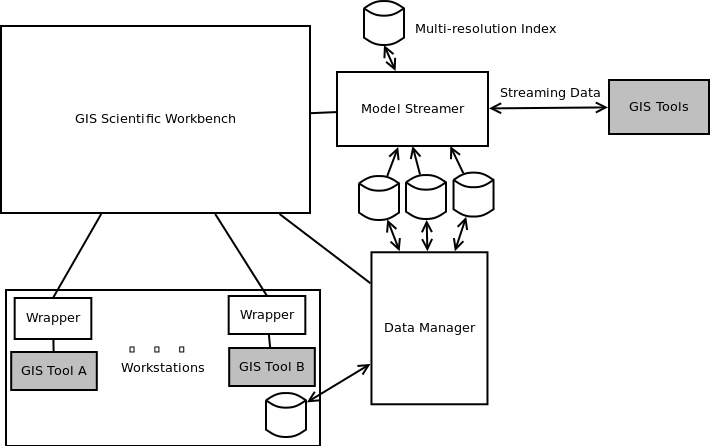
\includegraphics[width=0.8\textwidth]{projectDiagram.png}
    \caption{Interface between various project components}
\end{figure}

\section{Problem Statement and Research Questions}
This project aims to tackle two key issues faced by the Geomatics Department: the inability to interact with large models in real-time as well as the lack of tools enabling workflow to be automated. As such, the following key research questions have been proposed:
\subsection{Is it feasible to support real time viewing of models containing billions of points?}
The UCT Department of Geomatics has indicated that they have difficulties
handling the sizes of some of their models. These laser scanned models of
cultural heritage sites are often very large, some of them containing over
8 billion points. Given this vast scale of data, traditional viewing methods
and the current hardware and software systems are not able to cope.
Consequently, before viewing or manipulating the data, one must go through
a process of decimating the original data by a factor of 10, 100 or more.
This compromise is often unacceptable, as one may often require the full
original detail. This level of detail is often necessary for cultural heritage
sites in order to view details such as cracks and flaws, with a view to
preserving the site and preventing damage.

This project will investigate the feasibility of real-time interaction with the Zamani models in their full detail. Answering this research question in the affirmative would enable exploration of these models interactively without decreasing the resolution beforehand.
\subsection{How effective is an automated workflow system in the GIS context?}
Developing a geographic information system involves the capture, storage, manipulation, analysis
and management of geographic data. This data is very diverse and, as such, has to be handled
in quite diverse ways. The data gets abstracted into various forms. This presents a
rather unique challenge in managing the data as it could be used by anyone of the research
staff at any point in the process. Currently, data is being manually moved or copied to
where it is required. This takes up a lot of time, the movement is laborious, and it could benefit from automation.

Workflow Management Systems aim to decompose complicated projects and processes into
small atomic chucks \cite{Taylor:2006:WES:1196459}. This decomposition can then be
optimised to improve the efficiency.
GIS research projects generally have multi-person teams where the work is
done in a parallel fashion. Under these conditions workflow management systems
are particularly effective.

The aim is to provide a workflow management that is applicable for GIS projects.
This system should be able to: interface with the current systems, track and
manage the workflow, provide local data availability and content delivery, and
increase overall efficiency within the discipline.

\section{Procedures and Methods}
Given the above problems, the following procedures and methods are being proposed:
\subsection{Implement a Hierarchical Data Structure}
From researching the literature it seems that the most common way of dealing
with large point based models containing billions of points is to build a
multiresolution data structure to divide the model into manageable chunks.
Initially, only a small subset of the number of available points is required.
As one zooms into the model, additional points are fetched from the
data structure until the full original detail is available. Using such a
level-of-detail structure should enable the Department of Geomatics to
view even very large models at interactive frame rates, without having
to decimate the original data.

The data structure being proposed is an octree \cite{interactivepointclouds}. All
data is stored in the leaf nodes and inner nodes provide simplified multi-resolution
representations. Additionally the data structure imposes the constraint that no leaf
node should contain more than a specified number of points. This number of points is
a parameter in the system which will need to be determined experimentally, but for
this structure a value of around 30,000 was found to give good performance
\cite{interactivepointclouds}. The following figure shows the first three levels in such an octree structure, for a given point based model of a sphere.
\begin{figure}[h!]
\centering
    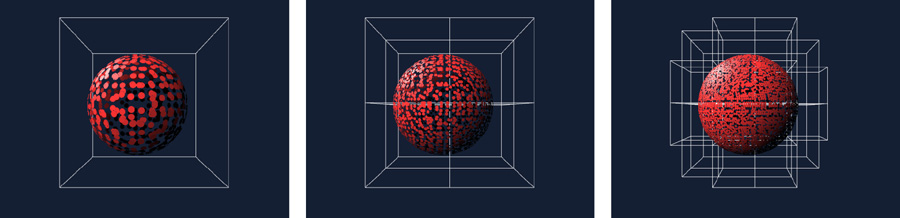
\includegraphics[width=0.5\textwidth]{oct.png}
    \caption{Each level of the octree structure provides greater detail}
\end{figure}

\subsection{Use an existing workflow management system as a base}
Various platforms already exist that are designed to manage workflow. These
systems, however, need to be adapted for GIS research. As these systems already
have a large number of features, such as, flow building toolkits, flow optimisation,
integration capabilities and monitoring, writing such a system
from the ground up would be a pointless task.

The decision on which system to use is partly dependent on the requirements
of the Geomatics department. This will be assessed and discussed. After
this decision is made the core functionalities would be established.

These components would then be implemented in a modular fashion, on top of
the existing system. The goal of these components is to address the core
functionalities that were determined.

The aim is to develop a system that integrates with  the current GIS
tools. A high level of collaboration with the Geomatics department will
be required. The feedback will be used to prioritise components and
functionalities.


\subsection{Testing and Evaluation}
A key evaluation criteria will be to demonstrate that the new
system is able to render the large point based models in real-time. Since this
functionality was not available previously, it will be a significant success.
Additionally, it will be important to test whether real-time streaming from the
server to client machines is feasible.

Further testing and refinement is required for the workbench
to determine the  following: the speed of the content
delivery system, the effectiveness of imposed workflow, the
effectiveness of the user interface and overall system stability.

\section{Ethical, Professional and Legal Issues}
\subsection{User Testing}
One of the components of the project involves the design and evaluation
of a user interface. Ideally, the design process for this would require
input from the user as well as testing. This testing requires that ethical clearance
be obtained.
\subsection{Data Privacy}
The Department of Geomatics has indicated that some of the data collected by
the Zamani Project is sensitive and is not to be made freely available. It is
important to ensure that, during the course of this project, this wish is respected
and that nothing is done to compromise the privacy of sensitive data. As such, the
data, once received, will only be stored on the server used as part of the project.
Special permission will be required if the data is requested for testing at an
external location.



\section{Related Work}
\subsection{Hierarchical Data Structure}
Common methods for structuring 3D data include octrees \cite{interactivepointclouds},
R-trees \cite{rtree}, bounding sphere hierarchies \cite{qsplat}, and Hilbert Space
Filling Curves \cite{hilbert}, each with their own advantages and disadvantages. Based
on the experimental results of each method, a dynamic octree structure seems to have
the best performance \cite{interactivepointclouds}. Wand et al. demonstrated its
ability to handle large models efficiently by using this data structure to achieve
interactive walkthroughs of a data set containing over 2.2 billion points.

\subsection{Automated Workflow Management}
Various fields of science have benefited from automated workflow. It has
seen good increases in productivity \cite{Brahe:2007:SWW:1316624.1316661} and the ability to share
workflow between colleges has aided quite significantly in th the reproducibility
of the science\cite{4721191}. GIS has been evaluated to be highly applicable to
workflow systems\cite{migliorini2011workflow}. However, some limitations were noted. Various components, such as the modeling and processing of spatial data,
would need to be added to make it feasible.

\section{Anticipated Outcomes}
There are two key anticipated outcomes from this project. First is the
implementation of a multi-resolution data structure to enable real-time interaction
with large point based models. Second is the development of a software system to
enable automated GIS workflow. It is expected that if both of these outcomes are
achieved, the results could have a significant impact in the Department of
Geomatics. It will enable the viewing of models in full detail without decimation
and could greatly increase the efficiency in Geomatics research. Key evaluation
criteria are:
\begin{itemize}
\item Can the system render the largest of the Zamani models at interactive frame rates?
\item Does the system enable streaming of large models from a central server?
\item Has dataflow been automated to provide transparent local access?
\item Has Geomatics research been successfully mapped to a workbench environment?
\end{itemize}

\section{Project Plan}
\subsection{Risks}
\subsubsection*{Request for Hardware Denied}
\noindent \textit{Severity: } High \\
\noindent \textit{Likelihood: } Low \\
It is possible that the request for a server will be denied. If this happens,
a considerable amount of restructuring will be required and it would have a
significant impact on the course of the project.
\subsubsection*{Network Constraints}
\noindent \textit{Severity: } Medium \\
\noindent \textit{Likelihood: } Low \\
One of the core functionalities of the system would be to provide
content delivery of data that is required for a specific task. Providing
this local data allows the task to get completed without unnecessary
fetching delays. There is a risk that this content delivery system
could saturate the network. This would cause the system to be slow
and unusable.
\subsubsection*{Middleware}
\noindent \textit{Severity: } High \\
\noindent \textit{Likelihood: } Low \\
For this project to be successful, the workflow management system will have to interface
heavily with existing software used to perform GIS operations. This will
require large amounts of middleware to be developed that understand
the input and output formats of this software. Since many of these
formats are proprietary, a significant amount of effort will have to
be made for the system to function. If these formats can not be integrated,
it presents a huge risk to the project.
\subsubsection*{Hardware Limitations}
\noindent \textit{Severity: } Medium \\
\noindent \textit{Likelihood: } Medium \\
There is a risk that the hardware available will not be able to cope
with the load that will be required. Since a distributed system is
not being proposed, there is a risk that the system will become a bottleneck. In
such an eventuality either the scale of the project would have to be decreased, or
a solution would have to be proposed. Such a solution would most likely involve
distributing the data on multiple servers.
\subsubsection*{Large Indices}
\noindent \textit{Severity: } Medium \\
\noindent \textit{Likelihood: } Low \\
When indexing the models, a significant amount of data will be generated.
Given that many of the models are already very large, these indices might
become infeasibly large. Dealing with such large indices will be an important
part of the project and this risk will have to be handled carefully.
\subsubsection*{Integration with Existing GIS Software}
\noindent \textit{Severity: } Low \\
\noindent \textit{Likelihood: } Medium \\
The hierarchical data structure required as part of this project aims to facilitate level
of detail streaming and real-time interaction. However, ideally, one should not have to
re-implement tools which are already available, such as ArcGIS. The aim is to integrate
the data structure into a pre-existing software package to prevent unnecessary work.
However, this may be difficult and there are several associated risks including
unavailability of source code and lack of documentation for the software.
\subsubsection*{Indexing takes too long}
\noindent \textit{Severity: } High \\
\noindent \textit{Likelihood: } Low \\
In the literature it had been noted that indexing the 3D data requires a significant
amount of time \cite{interactivepointclouds}. While it is hoped that this will not be
a problem, steps will have to be taken to ensure that the duration of the indexing
process does not pose a risk to the completion of the project. It will also be important
to allow time for the possible event of a system failure, in which case the indexing
process would have to be restarted.
\subsection{Timeline, including Gantt chart}
Figure~\ref{gant} shows the anticipated timeline in the form of a Gantt chart.
\begin{figure}[h!]
\centering
    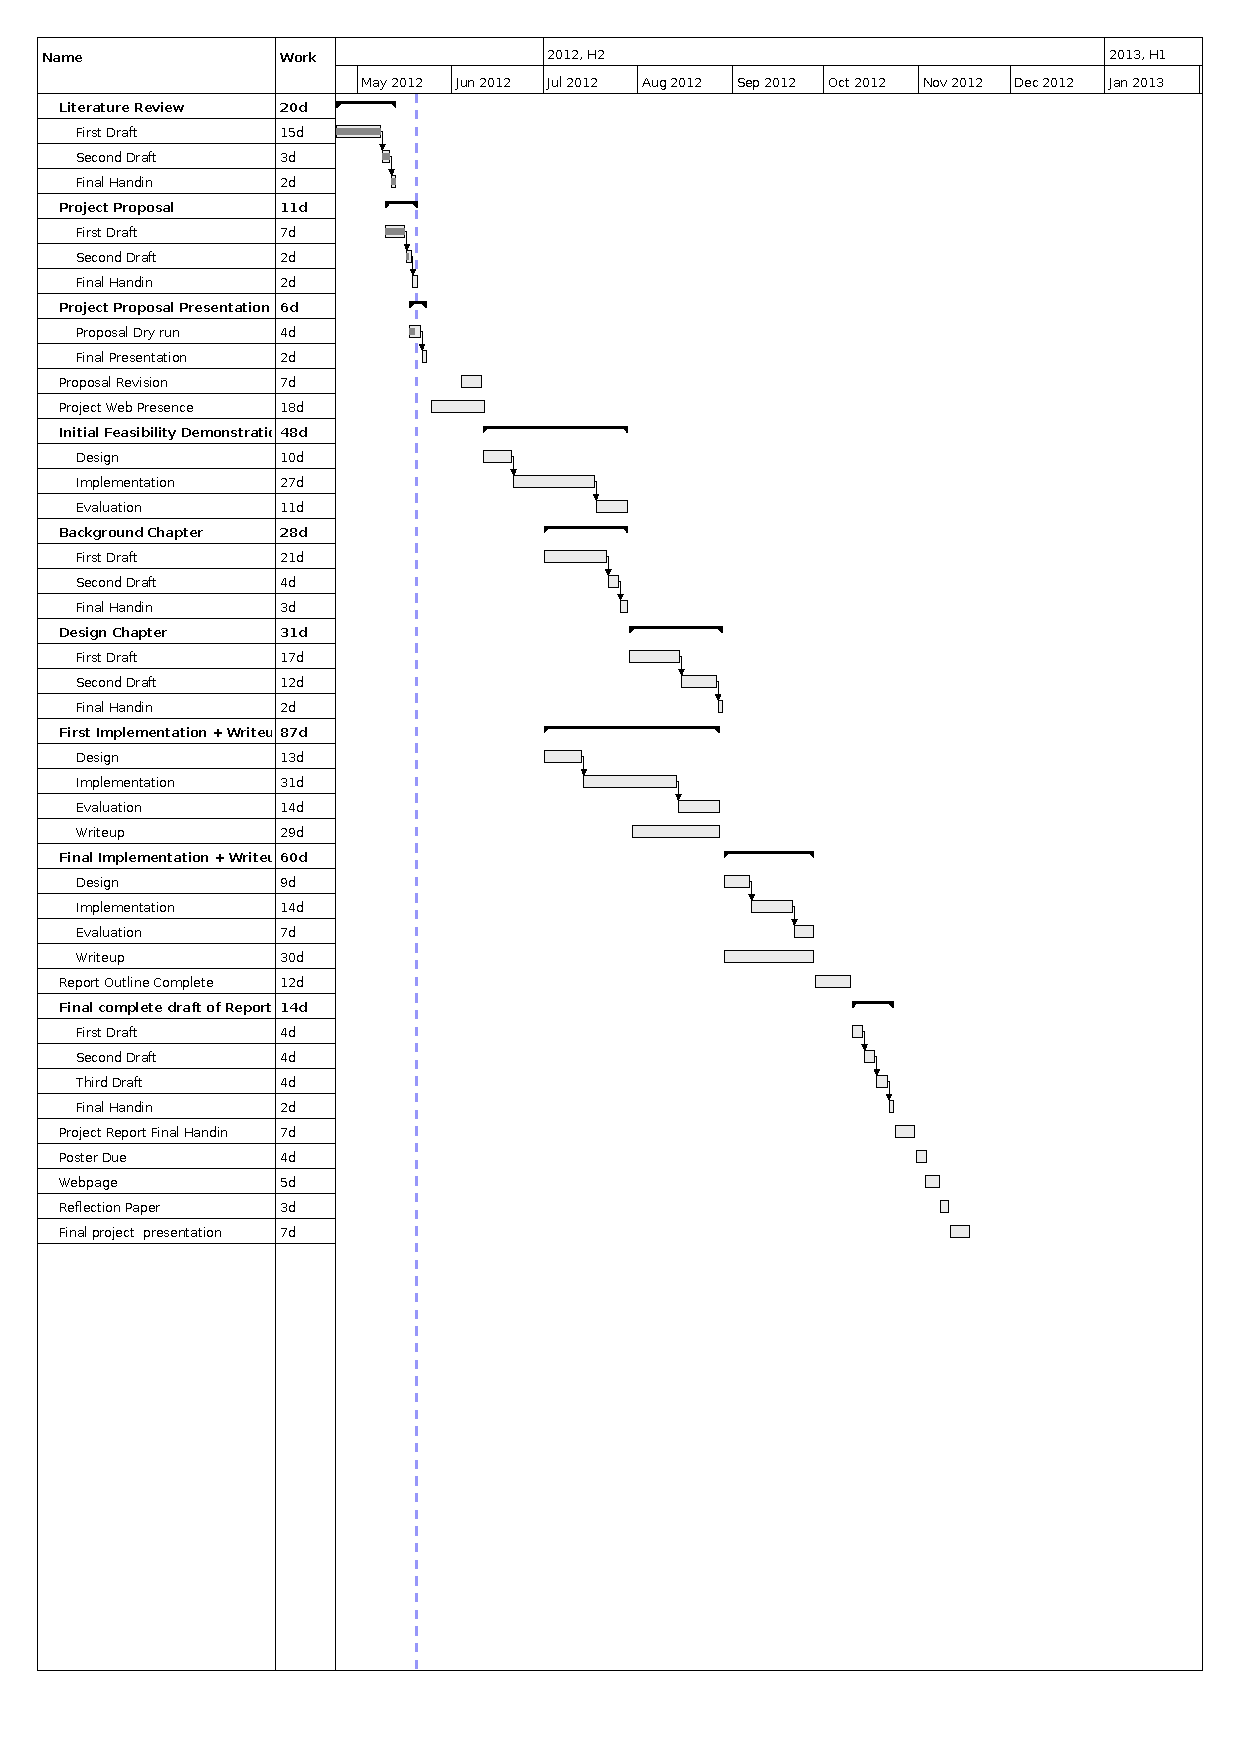
\includegraphics[width=1\textwidth]{gantt1.pdf}
    \caption{Project Schedule}
    \label{gant}
\end{figure}

\subsection{Resources required}
\subsubsection*{Hardware}
A server will be required for this project to enable central storage of the 3D models.
A large amount of storage will be required, as the Zamani data is over 20TB. The aim
is to initially store a subset of the data, and expand as the project progresses.
Multiple hard drives will be required and this will allow for a certain amount of
parallelism in data access. The exact specifications of the server are still
being finalised.
\subsubsection*{Geographic Data}
The Department of Geomatics has indicated that they are willing to make their data
available for the purposes of this project. It will be important to obtain the
models at an early stage as any delays in obtaining the models will delay the entire project.

\subsection{Milestones}
\subsubsection{Project Milestones}

\begin{tabular}{l||l|l|l}
    Description & Duration & Start & Finish \\
    \hline  \hline
    Literature Review & 18 days & 24 April 2012 & 14 May 2012 \\
    \indent Fist Draft Due & 15 days  & 24 April 2012  & 9 May 2012  \\
    \indent Second Draft & 3 days & 9 May 2012 & 12 May 2012 \\
    \hline
    Project Proposal & 12 days & 10 May 2012  & 21 May 2012 \\
    \indent First Draft Due & 7 days & 10 May 2012 & 17 May 2012 \\
    \indent Second Draft Due & 2 days  & 17 May 2012  & 19 May 2012 \\
    \hline
    Project Proposal Presentation & 6 days  & 18 May 2012 & 24 May 2012 \\
    \indent Proposal Dry run & 4 days & 18 May 2012 & 22 May 2012 \\
    \hline
    Proposal Revision Completed & 7 days & 4 June 2012 & 11 June 2012 \\
    \hline
    Project Web Presence & 18 days  & 25 May 2012 & 12 June 2012 \\
    \hline
    Initial Feasibility Demonstration & 48 days & 11 June 2012 & 29 July 2012 \\
    \indent Design & 10 days & 11 June 2012 & 21 June 2012 \\
    \indent Implementation & 27 days & 21 June 2012 & 18 July 2012 \\
    \indent Evaluation & 11 days & 18 July 2012 & 29 July 2012 \\
    \hline
    Background Chapter & 28 days & 1 July 2012  & 29 July 2012 \\
    \indent First Draft Due & 21 days & 1 July 2012 & 22 July 2012 \\
    \indent Second Draft Due & 4 days  & 22 July 2012 & 26 July 2012 \\
    \hline
    Design Chapter & 31 Days & 29 July 2012 & 29 August 2012 \\
    \indent First Draft Due & 17 days  & 29 July 2012 & 15 August 2012 \\
    \indent Second Draft Due & 14 days & 15 August 2012  & 26 August 2012 \\
    \hline
    First implementation and Writeup & 31 days & 1 July 2012 & 29 August 2012 \\
    \indent Design & 13 days & 1 July 2012 & 14 July 2012 \\
    \indent Implementation & 31 days & 14 July 2012 & 15 August 2012 \\
    \indent Evaluation & 14 days & 15 August 2012 & 26 August 2012  \\
    \indent Writeup & 29 days & 30 July 2012 & 29 August 2012 \\
    \hline
    Final implementation and Writeup & 30 days & 29 August 2012 & 28 September 2012 \\
    \indent Design & 9 days   & 29 August 2012  & 7 September 2012 \\
    \indent Implementation & 14 days & 7 Semptember 2012 & 21 September 2012 \\
    \indent Evaluation & 7 days & 21 September 2012  & 28 September 2012 \\
    \indent Writeup & 30 days & 29 August 2012 & 28 September 2012 \\
    \hline
    Report Outline Complete & 12 days  &28 September 2012 & 10 October 2012 \\
    \hline
    Final Complete Draft of Report & 14 days & 10 October 2012 & 24 October 2012 \\
    \indent First Draft Due & 4 days &10 October 2012 & 14 October 2012 \\
    \indent Second Draft Due & 4 days &14 October 2012 & 18 October 2012 \\
    \indent Third Draft Due & 4 days  &18 October 2012 & 22 October 2012 \\
    \hline
    Project Report Final Handin & 7 days & 24 October 2012 & 31 October 2012 \\
    \hline
    Poster Due & 4 days  & 31 October 2012 & 3 November 2012 \\
    \hline
    Website & 4 days & 31 October 2012 & 3 November 2012 \\
    \hline
    Project Demonstrations & 5 days & 3 November 2012 & 8 November 2012 \\
    \hline
    Write Reflection paper &3 days & 8 November 2012 & 11 November 2012 \\
    \hline
    Final project presentation & 7 days &11 November 2012 & 18 November 2012 \\

\end{tabular}
\subsection{Deliverables}
\subsubsection*{GIS Workbench}
A key component of the project is to produce a GIS workbench. This will
be the framework that ties all the components together. This will involve
using an existing Workflow System and setting it up to represent the
flow of a GIS project.
\subsubsection*{Middleware for Core Functionalities}
Once the GIS workflow is properly understood and modeled, it is
important to create middleware that interfaces with the systems that are
currently being used.
\subsubsection*{Data Flow Facilitator}
To be able produce the content delivery that is required, a dataflow
facilitator will need to be developed that is integrated with the
workflow management system.
\subsubsection*{Hierarchical Data Structure}
In order to facilitate level of detail streaming, it will be essential to
implement a hierarchical data structure that can support interactive
viewing of models containing billions of points.
\subsubsection*{Streaming Infrastructure}
A real-time streaming infrastructure from the server to client machines will be
an important deliverable. This will also need to be implemented as early as
possible.
\subsection{Work Allocation}
Timothy Trewartha will be implementing the hierarchical data structure to support
real-time interaction with the Zamani models. Michiel Johan Baird will be developing
the GIS workbench.




\bibliographystyle{apalike}
\bibliography{bibliography.bib}
\end{document}
